\IEEEoverridecommandlockouts
% The preceding line is only needed to identify funding in the first footnote. If that is unneeded, please comment it out.
\documentclass[conference]{IEEEtran}

\usepackage{amsmath,amssymb,amsfonts}
\usepackage{algorithmic}
\usepackage{graphicx}
\usepackage{textcomp}
\usepackage{xcolor}
\usepackage{comment}
\def\BibTeX{{\rm B\kern-.05em{\sc i\kern-.025em b}\kern-.08em
    T\kern-.1667em\lower.7ex\hbox{E}\kern-.125emX}}
\usepackage[numbers,sort&compress]{natbib}

\begin{document}

\title{How Does the Level of Somatosensory Feedback Fidelity Impact Motor Learning in VR: \\a Systematic Review}

\author{\IEEEauthorblockN{Reinprecht Christian}
\IEEEauthorblockA{TU Delft, NL \\
C.T.Reinprecht@student.tudelft.nl}
\and
\IEEEauthorblockN{Ratschat Alex}
\IEEEauthorblockA{TU Delft, NL \\
A.L.Ratschat@tudelft.nl}
\and
\IEEEauthorblockN{Marchal-Crespo Laura}
\IEEEauthorblockA{TU Delft, NL \\
L.MarchalCrespo@tudelft.nl}
}

\maketitle

\begin{abstract}
The abstract will come here. \\

\end{abstract}

\begin{IEEEkeywords}
motor learning, fidelity, virtual reality, systematic review
\end{IEEEkeywords}

\section{Introduction}

\begin{comment}
REWRITTEN FOR BETTER READABILITY:
Simulations in virtual reality (VR) provide a comprehensive platform for users to acquire new skills and competencies, as well as for the evaluation of their performance while being in a controlled and safe environment \cite{Harris2021ExploringSimulator}. In the virtual environment (VE), complex skills can be studied without giving up on experimental control, which facilitates the understanding of motor learning on a level that is not possible in the physical world \cite{Levac2019LearningReview}. 
Possible applications involve physical therapy and rehabilitation, sports training, education, marketing, telerobotics, and research, as well as gaming and entertainment \cite{Wu2023TrainingReality, Oagaz2022PerformanceReality}. Therefore it is not surprising that there is a great interest in VR-based training simulations, especially to teach skills that would otherwise have to be acquired in dangerous or sensitive environments, such as construction work, military training, or surgical operations \cite{Adami2021EffectivenessTeleoperation, Lele2013VirtualUtility, Qi2021VirtualScenario}.
\end{comment}

Simulations in virtual reality (VR) provide a comprehensive platform for users to acquire new skills and competencies, with applications ranging from physical therapy and rehabilitation to sports and industrial training, education, marketing, telerobotics, and research, as well as gaming and entertainment \cite{Wu2023TrainingReality, Oagaz2022PerformanceReality}. Furthermore, the virtual environment (VE) allows for the studying of complex skills, as well as the evaluation of the user's performance without giving up on experimental control, which facilitates the understanding of motor learning on a level that is not possible in the physical world \cite{Harris2021ExploringSimulator, Levac2019LearningReview}. Therefore it is not surprising that there is a great interest in VR-based training simulations, especially to teach skills that would otherwise have to be acquired in dangerous or sensitive environments, such as construction work, military training, or surgical operations \cite{Adami2021EffectivenessTeleoperation, Lele2013VirtualUtility, Qi2021VirtualScenario}.

When interacting with real-world objects, we do not only rely on visual feedback but also require information obtained through the mechanoreceptors in our skin \cite{AlexandreL.Ratschat2024EvaluatingStudy}. Exposing the user to somatosensory feedback, which includes sensations such as pressure, vibration, temperature, and the position and movement of body parts, may offer a promising approach to increase the effectiveness of motor learning \cite{Sainburg2022MovementNeurorehabilitation, Sigrist2013AugmentedReview}.
How closely the feedback resembles the real-world interaction in VR is defined by its fidelity \cite{Caird1996PersistentTraining}, ranging from simple vibration cues to high-fidelity feedback that feels like the user is interacting with a real object \cite{Yang2023TheSimulation}.  

While researchers previously assumed that higher fidelity correlates with better training performance in VR \cite{Caird1996PersistentTraining, Waller1998TheTraining}, recent research suggests that there is no linear correlation between the level of fidelity and motor performance: Instead, motor performance in a locomotion task was worse in conditions that yielded mid-fidelity, compared to scenarios with high fidelity and well-designed low fidelity \cite{MahdiNabiyouni201520153DUI.}. 

High-fidelity feedback can enhance the feeling of immersion and embodiment --- the experience that one's virtual avatar and one's actual body are indistinguishable \cite{Kilteni2012TheReality} --- and therefore significantly reduce perceptual strain on the subjects by making the interactions within the VE more intuitive \cite{Yang2023TheSimulation}. However, high levels of embodiment may adversely affect motor performance when the sensory feedback received is incongruent with anticipated stimuli, as this may increase the discrepancy between the perceived and actually executed movements \cite{Odermatt2021CongruencyReality}.
On the other hand, high levels of embodiment, coupled with congruence of (multi)sensory feedback, may offer an effective method for enhancing motor learning and performance \cite{Odermatt2021CongruencyReality}. 

When performing a motor learning task, using a mid-fidelity controller is associated with lower task complexity, effectively reducing the task load \cite{Yang2023TheSimulation}. This may be beneficial for the motor learning performance of people with impaired motor skills \cite{Sigrist2013AugmentedReview}, aligning with the challenge point framework which states that less skilled subjects might not advance if the performed task is too demanding \cite{Guadagnoll2004ChallengeLearning}. \\

\begin{comment}
An important aspect of a VE simulation is its level of immersion, i.e. the ability to create a realistic and enveloping experience that engages the human senses in a way that mimics real-world interactions \cite{Sanchez-Vives2005FromReality, Slater2016EnhancingReality}. By exposing the user to somatosensory feedback when interacting with objects in VR, one's feeling of presence in the virtual environment can be enhanced, i.e. the person's mental state of physically being in the VE \cite{Draper1998Telepresence, Dzardanova2024ExploringReality}. 

By studying immersion, researchers have explored the effect of different levels of fidelity in VR \cite{Mcmahan2012EvaluatingGame}, which is defined by how closely the physical simulation matches the operational environment \cite{Caird1996PersistentTraining}. 
While researchers previously assumed that higher fidelity correlates with better training performance in VR \cite{Caird1996PersistentTraining, Waller1998TheTraining}, recent research suggests that there is no linear correlation between the level of fidelity and motor performance: Instead, motor performance in a locomotion task was worse in conditions that yielded mid-fidelity, compared to scenarios with high fidelity and well-designed low fidelity \cite{MahdiNabiyouni201520153DUI.}. In a motor learning task, high fidelity can however significantly reduce perceptual strain on the subjects by making the interactions within the VE more intuitive, while using a mid-fidelity controller is associated with lower task complexity \cite{Yang2023TheSimulation}. This reduction of task load may especially be beneficial for the motor learning performance of people with impaired motor skills \cite{Sigrist2013AugmentedReview}, aligning with the challenge point framework which states that less skilled subjects might not advance if the performed task is too demanding \cite{Guadagnoll2004ChallengeLearning}.

% Embodiment: 
% - body ownership (vr body belongs to oneself)
% - agency (being in control of one's own actions)
% - self-location (experienced location of body in space)

High fidelity can enhance immersion and embodiment, which is the experience that one's virtual avatar and one's actual body are indistinguishable \cite{Kilteni2012TheReality}. However, high levels of embodiment may adversely affect motor performance when the sensory feedback received is incongruent with anticipated stimuli, as this may increase the discrepancy between the perceived and actually executed movements \cite{Odermatt2021CongruencyReality}. 
On the other hand, high levels of embodiment, coupled with congruence of (multi)sensory feedback, may offer an effective method for enhancing motor learning and performance \cite{Odermatt2021CongruencyReality}. 
\end{comment}

Since supplying high fidelity to a VE is very costly, it is important to determine in which scenarios low-fidelity feedback, such as through somatosensory cues, is sufficient and under which circumstances high-fidelity feedback is necessary. In this work, we aim to systematically review current research on the impact of different levels of somatosensory feedback on motor learning in VR. Furthermore, this review will address how the level of feedback fidelity may affect the transfer of the learned skills to the real environment.

We hypothesize that in complex movements that necessitate precise timing for the correct execution of the task, such as ballistic movements, a high level of somatosensory feedback fidelity may be beneficial for motor learning. However, in scenarios involving constant movement velocities, low-fidelity feedback may be sufficient for enhancing motor learning performance, allowing for reduced system cost and simpler experimental design. \newpage

\section{General Notes}

\subsection{Introduction structure:}
\begin{enumerate}
    \item Motivation
    \begin{enumerate}
        \item Learn new skills in VR
        \item Evaluate movements in VR
    \end{enumerate}
    \item Aspect of VR: level of immersion
    \begin{enumerate}
        \item Increases embodiment
        \item Enhances motor learning 
        \item By studying it, researchers have explored the effects of fidelity
        \begin{itemize}
            \item display fidelity
            \item interaction fidelity
        \end{itemize}
    \end{enumerate} 
    \item Cues and high fidelity to increase immersion
    \item Mid-fidelity worse than low- or high-fidelity
    \begin{itemize}
        \item Also include \textit{uncanny valley} effect here?
    \end{itemize}
\end{enumerate}
\vspace{5mm}

\section{Methods}

Using PRISMA method ...

\subsection{Eligibility criteria}
\subsubsection{Inclusion criteria}
To be eligible for inclusion, studies needed to focus on the impact of haptic and/or somatosensory feedback on motor learning in humans. There were no publication date or language limits. The databases Scopus, IEEE Xplore and PubMed were used for this review.

\subsubsection{Exclusion criteria}
Studies were considered not eligible for inclusion if they were focused on:
\begin{itemize}
    \item Studies not related to motor learning in humans,
    \item Systems not providing haptic feedback in VR,
    \item Studies that focused on a neurological condition and its implications for motor learning,
    \item Studies explaining a new assessment system for the evaluation of motor learning.
\end{itemize}



\begin{figure}[ht]
    \centering
    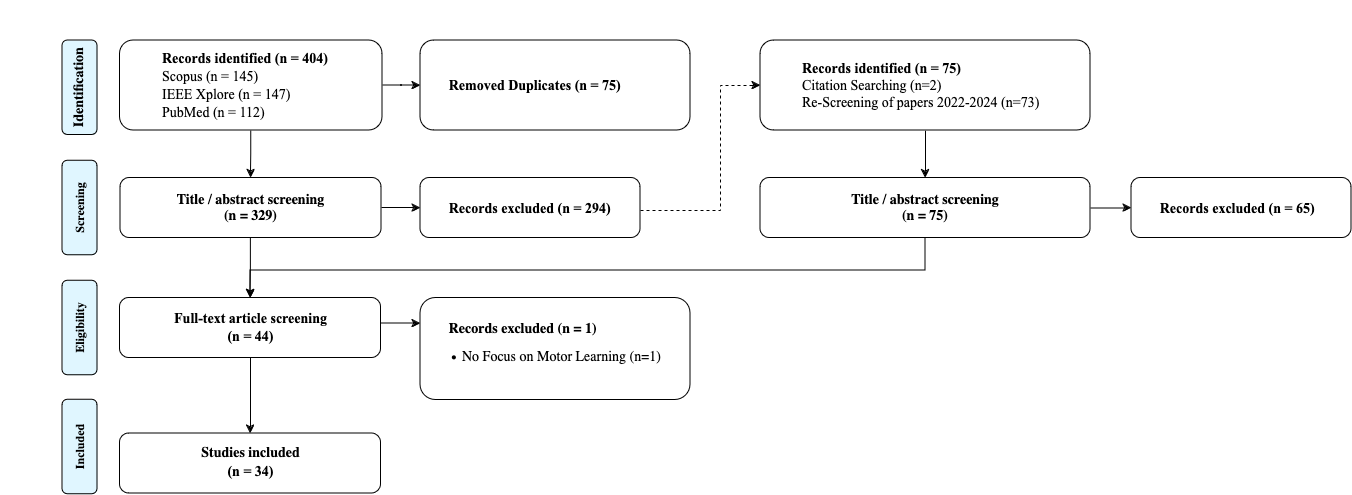
\includegraphics[width=\columnwidth]{prisma_overview.png} 
    \caption{Overview of the methodology using the PRISMA method}
    \label{fig:my_label}
\end{figure}


\subsection{Taken out from introduction}
\subsubsection{Sensory perceptions in VR}
Suppose that our sensory perceptions are replaced in the virtual environment by providing a natural visual scene, mimicking the interaction forces with the virtual objects, recreating the sound of the interaction, and possibly even the smell of the environment, then the perceptual model we create of our environment will be inferred from the actual stream of sensory data. This stream of sensory data is the virtual environment, and even though we know it is not real, our consciousness is completely transferred into it \cite{Slater2016EnhancingReality}. 

\subsubsection{Embodiment in VR}
The congruence between the physical stimulation of the biological body and the seen stimulation of one's body in VR will also enhance the sense of body ownership. Aside from the sense of self-location and agency --- which can be achieved by using a head-mounted display with a high frame rate and mapping one's limbs to the virtual body in near real-time --- body ownership is pivotal for achieving embodiment:  the experience that one's virtual avatar and one's actual body are indistinguishable \cite{Kilteni2012TheReality}.

\subsection{Also interesting}
Spatial tactile localization depends on sensorimotor binding: preliminary evidence from virtual reality. After the VR task, compared to the baseline condition, the point of subjective equality (PSE) shifted toward the hand that received the haptic feedback during the interaction (toward the right hand for the congruent condition and toward the left hand for the incongruent condition)\cite{Girondini2024SpatialReality}


\subsection{Mid-fidelity feedback}
Recent research has shown that motor performance was worse in conditions that yielded mid-fidelity \cite{MahdiNabiyouni201520153DUI.}.
Some researchers even compare this dip in performance to the uncanny valley effect first hypothesized by Mori \cite{Mori2012TheValley}, which describes the phenomenon that as robotic likeness to humans increases, our affinity to the robot increases as well, until there is a sharp drop at which the near-identical resemblance to a human being arouses a sense of unease \cite{Bhargava2018EvaluatingSimulations}. Finally, our affinity towards the robot recuperates again as human likeness increases further, and so does the motor performance with high fidelity due to the realism of the VE. 



\begin{comment}
\subsection{Questions that should be answered in the literature research:}

\begin{itemize}
    \item How does high fidelity compare to queues impact motor learning in Virtual Reality? Is learning better/more efficient with queues or with high fidelity?
    \item (On top of motor learning: Can the skills learned in the VE be applied in the real environment? What are the differences here if learning with queues vs with high fidelity?)
    \item Background:
    \begin{itemize}
        \item What are queues in the context of motor learning in VR?
        \item What is high fidelity in the context of motor learning in VR?
    \end{itemize}
\end{itemize}

\subsection{Motor Learning}

"After exploring the literature, we conclude that there is a notable lack of
conclusive research on what contributes to the success of IVR-based training. The works in
the literature are in an initial phase where the research focuses on measuring how the user
feels during the training rather than more advanced topics such as studying whether the
competencies acquired through virtual training translate to real-world performance." \cite{Narciso2021}.
- Maybe it's interesting for the thesis then?

"Participants also indicated that \textbf{haptic
feedback was beneficial in their ability to assemble virtual
products} and the majority of the participants preferred
using at least one haptic device." - \cite{Carlson2016}

"The results revealed that there
was \textbf{no significant difference in performance} between the
five treatment conditions. However, half of the participants
chose the 5DT Data Glove and the haptic-enabled Phantom
OmniÒ as their preferred device configuration." - \cite{Carlson2016}

\subsection{Fidelity in weight perception}
Vibrotactile feedback is a method to accurately render the perceived dynamics of the object in VR: "Vibrotactile feedback provides the opportunity for delivering dynamic cues rendering many different contact properties, such as impacts, object vibrations or textures." \cite{Cabaret2023}. \\

Experiment with high- vs low fidelity device in VR:
"Finally, even though quantitative results did not suggest that high fidelity haptic feedback positively influenced the participants' experience, many did think it added to the realism and naturalness, as indicated by their responses to the open-ended questions posed after exposure to all three conditions." \cite{Ryge2017EffectSimulation}.

Problem: in other papers not compared to low fidelity, for example in: \textit{Performance Benefits of High-Fidelity Passive Haptic Feedback in Virtual Reality Training}

\subsection{Other}

In the current consumer market, Virtual reality experiences are predominantly generated through visual and auditory feedback. Haptics are not yet well established, but are increasingly introduced to enhance the user’s sense of ‘reality’. With haptic (vibrotactile) feedback now part of the built-in mechanism of VR consumer devices, there is an urgent need to understand how different modalities work together to improve the user experience. This paper reports an experiment that explores the contributions made to participants’ sense of presence by haptic and visual feedback in a virtual environment. Participants experienced a virtual ball bouncing on a virtual stick resting across their avatar hands. We found that presence was enhanced when they could both see and feel the ball’s action; with a strong suggestion that haptic feedback alone gave rise to a greater sense of presence than visual alone. Similarly, while visual or bimodal feedback enhanced participants’ ability to locate where the ball bounced on the stick, our results suggest that the action itself was more readily discerned haptically than visually \cite{Gibbs2022AReality}. \\

Most virtual reality (VR) applications rely on auditory and visual stimulation, limiting how well the user experience can be. This systematic review looks at multisensory VR systems that incorporate haptic, olfactory, and gustatory cues, in addition to audio-visual. It aims to provide a broad overview of how multisensory stimulation affects VR experiences and to identify which types of sensory stimuli are most commonly used in the multisensory context. The authors found that 90 percent of the studies they examined showed a positive effect of multisensory VR, with haptics attracting considerable attention (65 percent). They highlight the need to devote more research and development to smell and taste, as they can add significant value to VR and user experiences \cite{Apostolou2022AReality}. \\

\subsection{Ideas}
\begin{itemize}
    \item Weight perception on the forearm is an interesting topic.
\end{itemize}
\end{comment}

\bibliographystyle{IEEEtran}
\bibliography{references}


\end{document}
